\documentclass[14pt]{extarticle}

\usepackage{microtype}
\usepackage[T1]{fontenc}
\usepackage[utf8]{inputenc}
\usepackage[round]{natbib}
\setlength{\bibhang}{0pt}
\usepackage{graphicx}
\DeclareGraphicsExtensions{.pdf, .png, .jpg}
\usepackage{extsizes}
\usepackage{amsmath}
\usepackage[version=3]{mhchem}
\usepackage{booktabs}
\usepackage[ddmmyyyy]{datetime}
%\usepackage{setspace}
%\setstretch{1.5}
\usepackage{authblk}
%\usepackage{lineno}
%\linenumbers
\usepackage{array}
\usepackage{todonotes}
\usepackage[a4paper, margin=25mm]{geometry}
\newcolumntype{P}[1]{>{\raggedright\let\newline\\\arraybackslash}p{#1}}
\newcolumntype{M}[1]{>{\raggedright\let\newline\\\arraybackslash}m{#1}}
\usepackage[hidelinks,pdftex,
           pdfauthor={Jane Coates},
           pdftitle={Sensitivity of Modelled Tropospheric Ozone to VOC Emission Inventories},
           pdfsubject={Solvent Emissions},
           pdfkeywords={TOPP, solvent emissions, emission inventories, boxmodel, Ox production, atmospheric chemistry},
           pdfproducer={Latex with hyperref},
           pdfcreator={pdflatex}]{hyperref}

\sloppy

\title{Sensitivity of Modelled Tropospheric Ozone to VOC Emission Inventories}
\author[1]{J. Coates}
\author[1]{E. von Schneidemesser}
\author[2]{Hugo Denier van der Gon}
\author[2]{Anton Visschedijk}
\author[1]{T. Butler}
\affil[1]{Institute for Advanced Sustainability Studies, Potsdam, Germany}
\affil[2]{TNO Built Environment and Geosciences, Utrecht, The Netherlands}
\renewcommand\Authands{ and }

\begin{document}

\maketitle

\begin{abstract}
    Volatile organic compounds (VOCs) are detrimental to human health both directly and indirectly, through their role in the formation of secondary air pollutants such as tropospheric ozone (\ce{O3}).
    The identity and amounts of VOCs emitted into the troposphere are represented in emission inventories (EIs) for input to chemical transport models that predict air pollutant levels.
    These EIs are outdated but before taking on the task of providing an up-to-date and highly speciated EI, the sensitivity of models to the change in VOC input needs to be addressed.
    We determine the sensitivity of modelled tropospheric \ce{O3} to VOC emission inventories by comparing the maximum potential difference in \ce{O3} levels using various solvent sector EIs in an idealised study using a boxmodel.
    We further test this sensitivity using three chemical mechanisms that describe \ce{O3} production chemistry at different scales -- point (MCM~v3.2), regional (RADM2) and global (MOZART-4).
    Under the conditions of our study, we find a maximum difference of 17~ppbv between different EIs of the solvent sector, reproduced by each chemical mechanism. 
    At the end of the seven-day model runs, alkanes have the largest contribution (up to $40$\%) to \ce{O3} production and the amount of total alkane emissions specified by the solvent sector emission inventories is directly related to the amount of \ce{O3} produced.
    These results indicate that modelled tropospheric \ce{O3} is sensitive to the distribution of VOCs specified by emission inventories and that the maximum amount of \ce{O_x} produced from an updated emission inventory depends on the amount of alkane emissions specified.
\end{abstract}

\section{Introduction}

Volatile organic compounds (VOCs) have an adverse effect on health, both directly and indirectly as a precursor of secondary air pollutants \citep{Laurent:2014}.
Tropospheric ozone (\ce{O3}) is one such secondary air pollutant formed from the degradation of VOC in the presence of nitrogen oxides (\ce{NO_x}) and sunlight \citep{Atkinson:2000}.
Numerical chemical transport models use emissions of NMVOCs (non-methane VOCs) and \ce{NO_x} to predict \ce{O3} concentrations.

Emission Inventories (EIs) allocate anthropogenic NMVOC emissions into sectors by source (e.g. industry, solvent use), these sectors are further sub-divided into individual NMVOC and groups of NMVOC with relative contributions to total sector emissions. 
Modelling studies may use EIs to determine the NMVOC species represented by the model and the amounts of emitted NMVOC.  
Despite EIs being widely used as model input, there are many uncertainties with EIs, such as discrepancies between the contributions of NMVOC specified by an EI and ambient measurements of the NMVOC \citep{Borbon:2013}, also EIs fail to capture the change in NMVOC emissions over time \citep{Boynard:2014}.

\citet{Li:2014} have compared the modelled tropospheric \ce{O3} produced from different EIs used over east Asia using multiple chemical mechanisms.
They calculate the ozone formation potential of individual NMVOC and determine that highly reactive VOC, such as ethene and reactive aromatic VOC, have the largest impact on tropospheric \ce{O3} production.

Improving an EI requires a large amount of effort due to the diverse sources and variety of inputs. 
Before undertaking such a task, it is valuable to know whether models are sensitive to changing NMVOC input.
In particular, how large are the differences in modelled \ce{O3} using different EIs as model input.

In this study, we address the sensitivity of modelled \ce{O3} to different EIs of the solvent sector; we consider the solvent sector as this has the largest contribution to NMVOC emissions \citep{AQEU:2011} and EIs for this sector specify differing NMVOC and relative contributions.
We calculate the maximum potential difference in modelled \ce{O3} produced by various solvent sector EIs using an idealised boxmodel setup.

\section{Materials and Methods}

\subsection{Solvent Sector NMVOC Emission Inventories}
Solvent sector EIs were chosen to represent a range of case studies, including the european average NMVOC speciation (TNO), a model specific speciation (EMEP), a general anthropogenic speciation (IPCC) and country specific profiles for Germany, Greece and the UK.
Two time-points of the Greek and UK profiles are included to represent the evolution of solvent sector NMVOC emissions over time.
Table~\ref{t:speciations} lists all these solvent sector EIs compared in this study.
\begin{table}
    \begin{center}
        \label{t:speciations}
        \caption{The solvent sector emission inventories compared in this study.}
        \begin{tabular}{lllP{5.2cm}}
            \toprule
            \textbf{Speciation} & \textbf{Comment} & \textbf{Reference} \\ \bottomrule
            TNO & European average &  \citet{Builtjes:2002} \\ \hline
            IPCC & Model Specific & \citet{Ehhalt:2001} \\ \hline
            EMEP & Model Specific & \citet{Simpson:2012} \\ \hline
            DE94 & Country Specific & \citet{Friedrich:2002} \\ \hline
            GR95 & Country Specific & \citet{Sidiropoulos:2007} \\ \hline
            GR05 & Country Specific & \citet{Sidiropoulos:2007} \\ \hline
            UK98 & Country Specific & \citet{Goodwin:2000} \\ \hline
            UK08 & Country Specific & \citet{Murrells:2010} \\ \bottomrule
        \end{tabular}
    \end{center}
\end{table}

\subsection{Model Description}
We use the MECCA boxmodel \citep{Sander:2005} as described in \citet{Coates:2015} without any meteorology or transport processes that are included in 3-D models to focus solely on the photochemical gas-phase processes that produce \ce{O3}.
Model runs were performed using the detailed gas-phase chemistry of the Master Chemical Mechanism (MCM~v3.2) \citep{Jenkin:1997, Jenkin:2003, Saunders:2003, Bloss:2005, MCM_Site}.

Reduced chemical mechanisms are used by 3-D models for reasons of computational efficiency and these reduced chemical mechanisms typically represent NMVOC by aggregating many VOC into a surrogate mechanism species (lumping).
Hence, changing the chemical mechanism in a model also changes the NMVOC input.
We also determined the sensitivity of modelled \ce{O3} mixing ratios using the MOZART-4 \citep{Emmons:2010} and RADM2 \citep{Stockwell:1990} mechanisms which are used for global and regional modelling studies, respectively.
\citet{Coates:2015} describes the implementation of MOZART-4 and RADM2 into the MECCA boxmodel.

\subsection{Model Setup and Simulations}
The model is run under equinoctical conditions representative of $34$ degrees North (roughly the city of Los Angeles, USA).
CO and \ce{O3} were initialised at $200$~ppbv and $40$~ppbv and then allowed to evolve freely, methane (\ce{CH4}) was fixed at $1.8$~ppmv.
In each model run, we used \ce{NO_x} conditions that induce maximum \ce{O3} production by emitting the amount of NO needed to balance the chemical source of radicals at each time step.

Model runs were performed using each of the solvent sector EIs of Table~\ref{t:speciations} using the three gas-phase chemistry schemes (MCM~v3.2, MOZART-4 and RADM2).
A further set of model runs was performed with each EI after ``tagging'' each of the chemical mechanisms for the emitted NMVOC.
This tagging approach followed \citet{Butler:2011} and \citet{Coates:2015} and allows attribution of \ce{O_x} production back to the emitted VOC.
As \ce{O3} production is dominated by rapid photochemical cycles, the \ce{O_x} family is used as a surrogate for \ce{O3} production.
We define the \ce{O_x} family to include \ce{O3}, \ce{NO2}, O, \ce{O^1D}, \ce{NO3}, \ce{N2O5} and other species that are involved in fast photochemical production and loss cycles with \ce{NO2}.

\subsection{NMVOC Initial Conditions}
This study considered an idealised urban area of 1000~km$^2$ with total NMVOC emissions of 1000~tons~day$^{-1}$ \citep{Warneke:2007}.
As the solvent sector contributes 43\% to total NMVOC emissions \citep{AQEU:2011}, the total amount of NMVOC emissions in each model run was 430~tons~day$^{-1}$.

The total NMVOC emissions were then allocated to the individual NMVOC and groups of NMVOC specified by the EIs in Table~\ref{t:speciations} that are represented by MCM~v3.2 species.
When an EI specified a group of NMVOC then \citet{Passant:2002} was used to determine the individual NMVOC and contributions of the specified group.
For example, the TNO EI specifies a contribution of $8$\% from xylenes; the contributions of the individual xylene isomers are listed in \citet{Passant:2002} and used to calculate the emissions of m-, o- and p-xylene in the TNO model run with MCM~v3.2 chemistry.  
The NMVOC emissions were held constant until noon of first day.

The initial NMVOC emissions and NMVOC species represented by the MCM~v3.2 were mapped to the MOZART-4 and RADM2 primary species based on the recommendations from the respective literature \citep{Emmons:2010, Stockwell:1990}.
The MCM~v3.2 species and respective emissions were aggregated into the MOZART-4 and RADM2 species by weighting the MCM~v3.2 emissions by the respective carbon numbers.
This approach ensured that the amount of emitted reactive carbon was same in each model run with the different chemistry schemes.

\section{Results and Discussion}

\subsection[Sensitivity of O3 and Ox Production Budgets]{Sensitivity of \ce{O3} and \ce{O_x} Production Budgets} \label{ss:o3}
\begin{figure}
    \centering
    \caption{Differences in the time series of \ce{O3} mixing ratios for each solvent sector EI using each chemical mechanism.}
    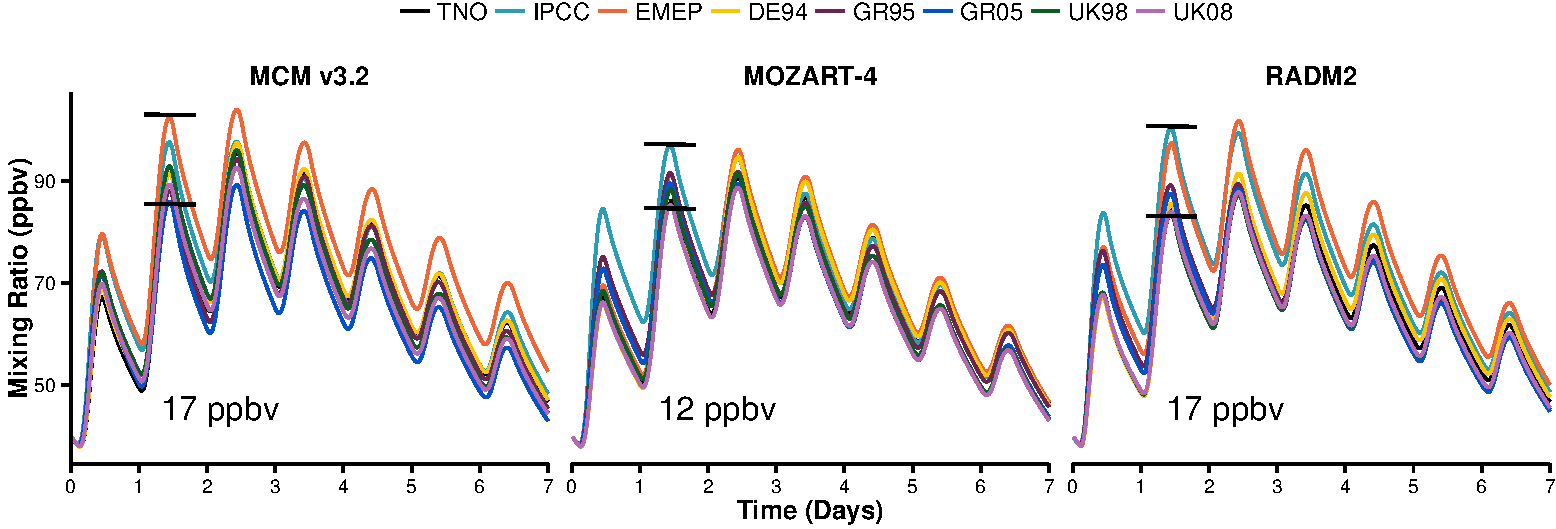
\includegraphics[width=\textwidth]{Scientific_Writing_Course/Pictures/Solvents_Only_O3_mixing_ratios}
    \label{f:O3_time_series}
    \vspace{-2mm}
\end{figure}
The sensitivity of modelled \ce{O3} to the NMVOC specified by the EIs listed in Table~\ref{t:speciations} with each chemical mechanism is shown in Fig.~\ref{f:O3_time_series} by comparing the time series of the \ce{O3} mixing ratios obtained in each model run.
The differences between the highest and lowest maxima of the second day \ce{O3} mixing ratios are 17~ppbv using MCM~v3.2, 12~ppbv in MOZART-4 and 17~ppbv with RADM2.
In general, the model specific EIs (IPCC and EMEP) produce the largest \ce{O3} mixing ratios in each chemical mechanism.

The time series of \ce{O3} mixing ratios obtained with the different EIs have a different spread in the reduced chemical mechanisms (MOZART-4 and RADM2) than the more detailed MCM~v3.2.
Using MOZART-4, the time series of \ce{O3} mixing ratios have a lower spread than the MCM v3.2 runs.
With RADM2, most speciations produce similar time series of \ce{O3} mixing ratios except for EMEP and IPCC which are higher than the rest.
These different spreads are due to the effect of lumping the emitted NMVOC from the MCM~v3.2 into the mechanism species specified by MOZART-4 and RADM2.
For example, the TNO solvent sector emissions are represented using $58$ MCM~v3.2 species but only $8$ are required by MOZART-4 and $7$ by RADM2.

\begin{figure}
    \centering
    \caption{The first day and cumulative \ce{O_x} production budgets at the end of the model run allocated to the groups specified by the EIs, showing which emitted NMVOC groups contribute the most to \ce{O_x} production.}
    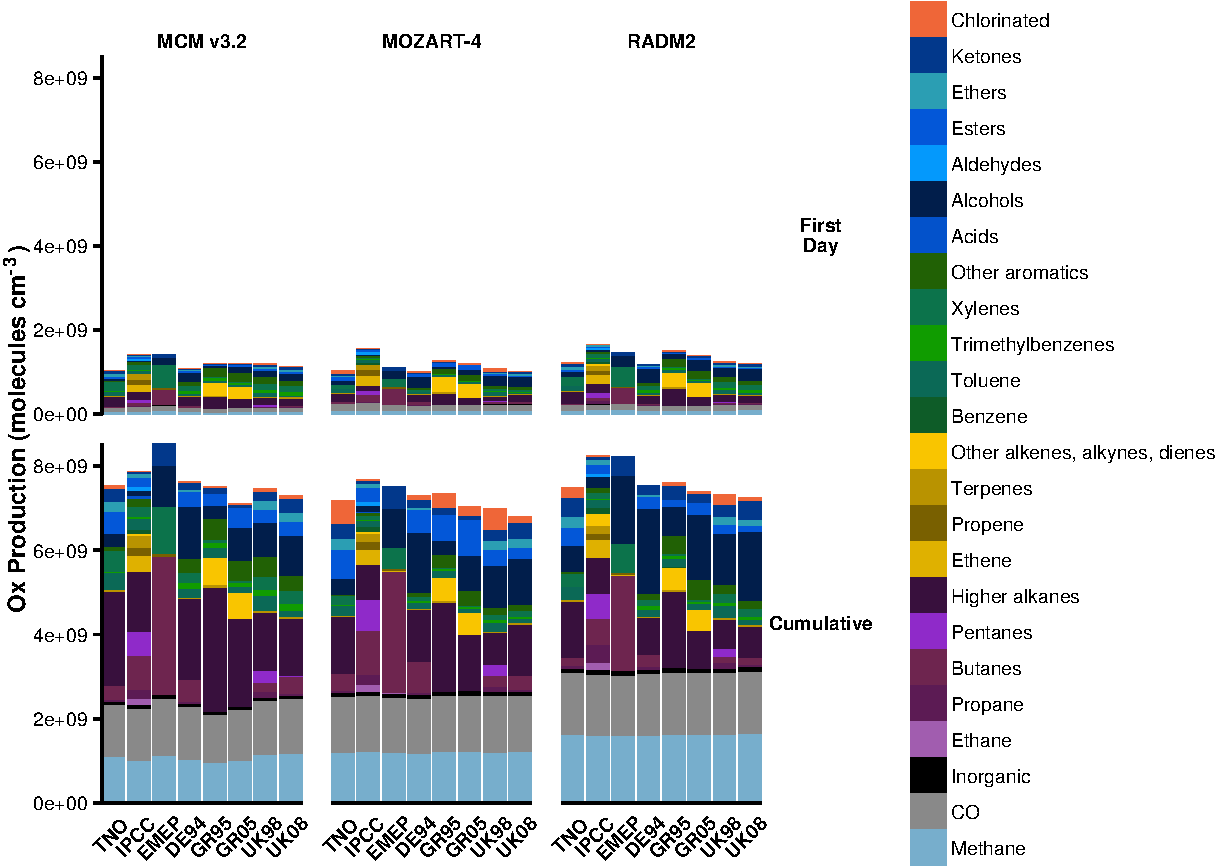
\includegraphics[width=0.9\textwidth]{Scientific_Writing_Course/Pictures/Cumulative_Ox_budget_allocated_facet_mechanism}
    \label{f:Ox_budget}
    \vspace{-2mm}
\end{figure}
In order to understand the differences in modelled \ce{O3} seen in Fig.~\ref{f:O3_time_series}, we show the first day and cumulative \ce{O_x} production budgets allocated to the NMVOC groups specified by the EIs (Fig.~\ref{f:Ox_budget}). 
This allocation is possible using the tagging approach which was previously used in \citet{Butler:2011} to allocate \ce{O_x} production to emitted NMVOC over Los Angeles and Beijing and in \citet{Coates:2015} to compare the \ce{O_x} produced over Los Angeles by several chemical mechanisms, including MOZART-4 and RADM2, to MCM~v3.2.

Figure \ref{f:Ox_budget} shows that \ce{O_x} production is influenced by different groups depending on the whether a model run of one day or multiple days is considered.
On the first day the more reactive species such as alkenes (ethene, propene, terpenes and other alkenes) and many aromatics (xylenes, trimethylbenzenes) that produce the most \ce{O_x}.
Whereas at the end of seven days, alkanes (ethane, propane, butane, pentanes and higher alkanes) have the largest impact on cumulative \ce{O_x} production (up to $40$\% of the total \ce{O_x} production budget).
This large contribution of alkanes to \ce{O_x} production during multi-day model runs is also seen in \citet{Butler:2011} and \citet{Coates:2015}.

\citet{Li:2014} compared modelled \ce{O3} produced from different EIs used over East Asia focusing on the representation of individual NMVOC between the EIs.
They calculate the ozone formation potential (OFP) of individual VOC by multiplying the fractional contributions of the VOC emissions from its source by the Maximum Incremental Reactivity (MIR) of the VOC.
MIR values were calculated in \citet{Carter:1994} using model runs of one day which emphasises the impact of reactive VOC which produce maximum \ce{O3} on the first day at the expense of less-reactive VOC such as alkanes that produce maximum \ce{O3} after the first day.
These results are consistent with our first day \ce{O_x} production budgets (Fig. \ref{f:Ox_budget}), however when considering multi-day model runs, alkanes have a higher potential to produce \ce{O3} \citep{Butler:2011, Coates:2015} which is also seen in Fig.~\ref{f:Ox_budget}.

The cumulative \ce{O_x} production from the different EIs between the chemical mechanisms (Fig.~\ref{f:Ox_budget}) show similar results to \citet{Coates:2015}.
Namely, that alkenes (ethene, propene, other alkenes, terpenes) produce similar amounts of \ce{O_x} between mechanisms while the \ce{O_x} produced from aromatics (benzene, toluene, xylenes, trimethylbenzenes and other aromatics) and alkanes (ethane, propane, butanes, pentanes and higher alkanes) is generally lower in the simplified chemical mechanisms (MOZART-4 and RADM2) than the MCM~v3.2.

\subsection{Alkanes and Ox Production}
\begin{figure}
    \centering
    \caption{Correlation of total \ce{O_x} production at the end of the model run to the fraction of alkanes emissions specified by each EI. The Pearson correlation coefficient, r, is also shown.}
    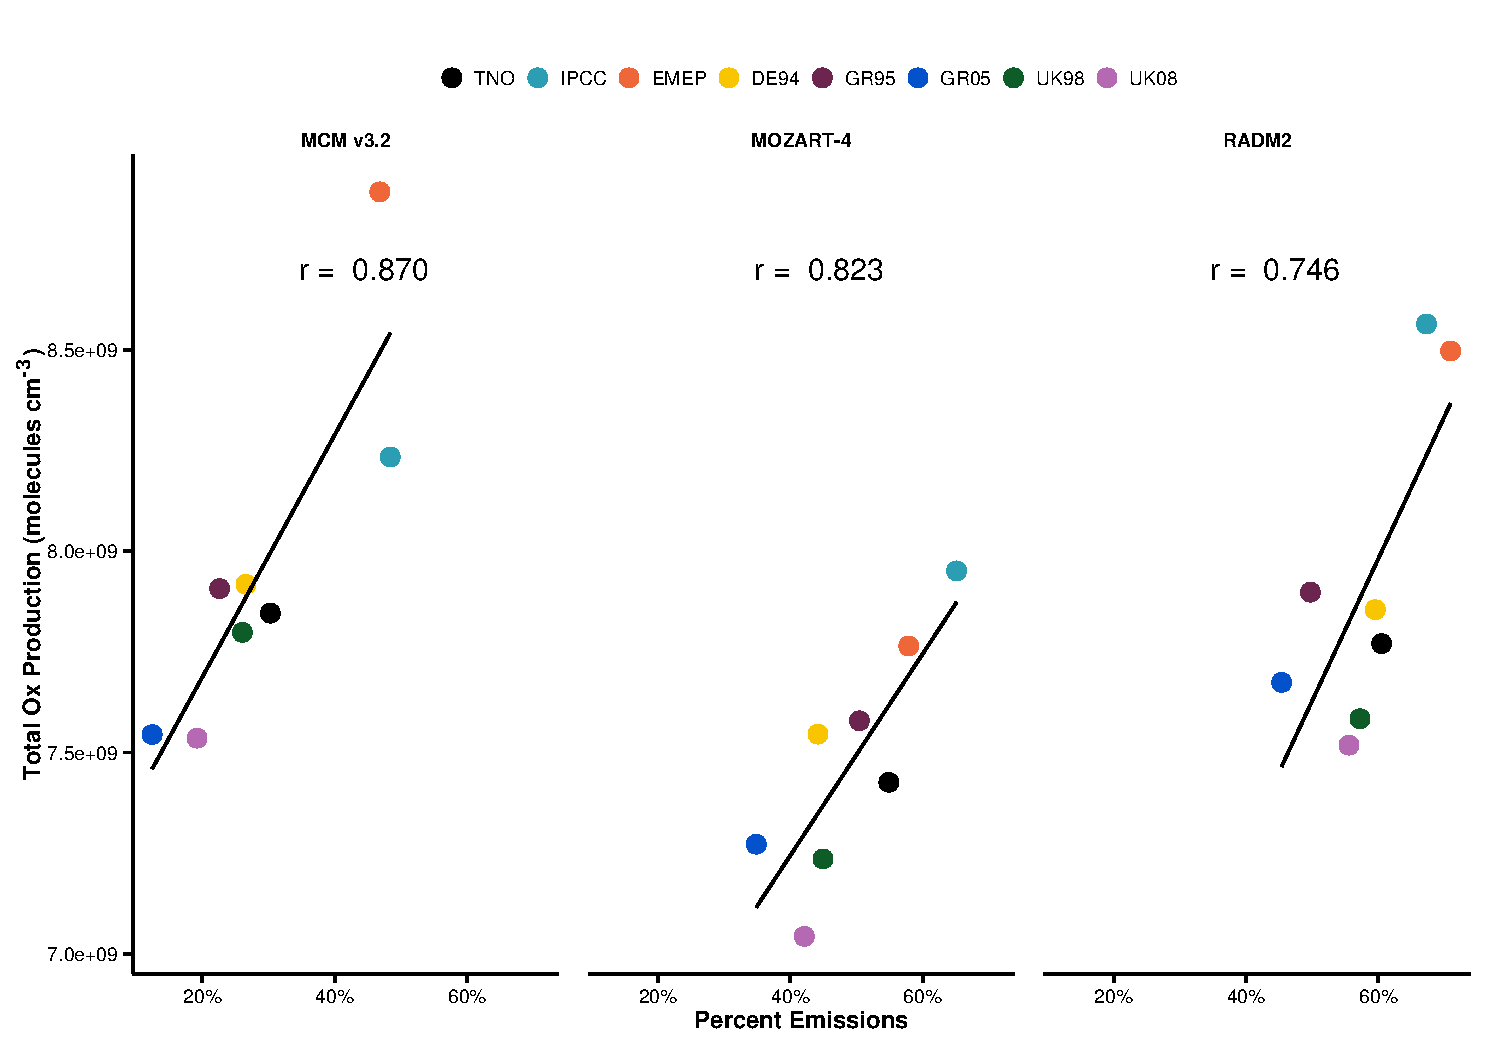
\includegraphics[width=0.9\textwidth]{Scientific_Writing_Course/Pictures/Ox_production_vs_type_emission_fraction_all_mechanisms}
    \label{f:correlations}
    \vspace{-2mm}
\end{figure} 
Section~\ref{ss:o3} showed that alkanes have the largest contribution to \ce{O_x} production after seven days.
%Moreover, the representation of alkanes in simplified chemical mechanisms impacts \ce{O_x} production as alkanes, especially larger alkanes, produce lower amounts of \ce{O_x} than the detailed MCM~v3.2 mechanism.
In this section, we further analyse the impact of alkanes on \ce{O_x} production by correlating the total amount of alkane emissions specified in each EI with the total \ce{O_x} produced in the model runs.  
This correlation between total \ce{O_x} production at the end of the model run and the percent of total alkane emissions is shown in Fig.~\ref{f:correlations}.
The Pearson correlation coefficients in Fig.~\ref{f:correlations} show that EIs specifying more alkane emissions produce more \ce{O_x}.
In particular, the model specific EIs (IPCC and EMEP) EIs specify larger alkane emissions than any other EI and in turn have the largest \ce{O3} mixing ratios in Fig.~\ref{f:O3_time_series}.

Solvent sector EIs that are based on ambient measurements specify a larger contribution from oxygenated NMVOC groups leading to lower \ce{O_x} production than EIs with larger alkane contributions.
Moreover, the more recent EIs for Greece and the UK specify a larger contribution from oxygenated NMVOC than the earlier version, and thus have lower contributions from alkanes.
These results indicate that solvent sector emissions are trending towards larger emissions from oxygenated NMVOC and that the EIs specified by the IPCC and EMEP models are out of date.

%\subsection[Ox Production in Reduced Mechanisms]{\ce{O_x} Production in Reduced Mechanisms}
%\begin{figure}
%    \centering
%    \caption{Time series of \ce{OH} mixing ratios obtained with each solvent sector EI using the different chemical mechanisms.}
%    \includegraphics[width=\textwidth]{Pictures/Solvents_Only_OH_mixing_ratios_facet_speciation}
%    \label{f:OH_time_series}
%    \vspace{-2mm}
%\end{figure}
%
%Comparing the \ce{O_x} produced from the same solvent sector EI but between the different chemical mechanisms used (Fig.~\ref{f:Ox_budget}) shows that more \ce{O_x} is produced from \ce{CH4} degradation in both MOZART-4 and RADM2 than in the more detailed MCM~v3.2.
%As \ce{CH4} is fixed throughout the model run, this indicates that more OH is produced during the model runs using MOZART-4 and RADM2 than the MCM~v3.2.
%This is the case as seen in Fig.~\ref{f:OH_time_series}, where for each solvent sector EI (except EMEP) higher OH mixing ratios are produced during the runs using MOZART-4 and RADM2 than MCM~v3.2.
%
%The same inorganic chemistry of MCM~v3.2 is used in each mechanism meaning that any differences in OH production results from the treatments of organic degradation chemistry in MOZART-4 and RADM2.
%The main source of OH production that can be directly attributed to organic degradration is through the reaction of \ce{HO2} and NO.
%\ce{HO2} is formed from the degradation of organic products and so its production can be attributed to the emitted VOC groups by using the tagged model runs similar to \ce{O_x} production budgets as in Fig.~\ref{f:Ox_budget}.
%
%\begin{figure}
%    \centering
%    \caption{Cumulative \ce{HO2x} production from each EI compared between the different mechanisms for the first four days of the model runs.}
%    \includegraphics[width=0.9\textwidth]{Pictures/Cumulative_HO2x_budget_allocated_facet_speciation}
%    \label{f:ho2x_production}
%    \vspace{-2mm}
%\end{figure} 
%To investigate the sources of \ce{HO2} production arising from organic degradation between the mechanisms for each of the solvent sector EI runs, the HO2x (= \ce{HO2} + \ce{HO2NO2}) production budgets have been attributed to the groups of emitted VOC specified by the EIs. 
%The daily HO2x budgets for the first four days of model runs are shown in Fig.~\ref{f:ho2x_production} as in Fig.~\ref{f:OH_time_series} it is during the first part of the model run that higher OH mixing ratios in MOZART-4 and RADM2.
%
%Figure~\ref{f:ho2x_production} shows that during the first part of the model runs, more \ce{HO2} is produced from the degradation of higher alkanes and esters in MOZART-4 and RADM2 for each solvent sector EI.
%The OH mixing ratios obtained during the EMEP model runs are very similar for each chemical mechanism (Fig.~\ref{f:OH_time_series}), and the EMEP does not specify any VOC emissions from higher alkanes (butanes are listed instead) and esters.
%Higher alkanes and esters are represented in both MOZART-4 and RADM2 by a lumped mechanism species which produces \ce{HO2} earlier in the model run than when using the dedicated analogous species of the MCM~v3.2 that represent higher alkanes and esters.
%In particular, the reaction of the peroxy radical formed from the initial OH-oxidation of the MOZART-4 and RADM2 species with NO immediately produces \ce{HO2}.
%Whereas, production of \ce{HO2} happens at a later stage during the MCM~v3.2 degradation.
%
%These results concur with those of \citet{Coates:2015}, in which they find that lumped mechanism species respresenting alkanes are broken down faster in reduced mechanisms than with the MCM~v3.2.
%This faster break down of the mechanism species leads to an earlier maximum in \ce{O_x} (and in turn \ce{HO2}) than the MCM~v3.2.

\section{Conclusions}
Our modelling study suggests that the choice of emission inventory speciation influences modelled tropospheric \ce{O3} mixing ratios.
Similar differences in modelled \ce{O3} are obtained using detailed gas-phase chemistry (MCM~v3.2) and simplified chemical mechanisms (MOZART-4 and RADM2).
We have shown that after model runs of seven days, alkanes have the largest contribution to the \ce{O_x} production budget.
Furthermore, the amount of \ce{O_x} produced is directly related to the amount of alkane emissions specified by the EI.

Emission inventories that are used specifically for model inputs (IPCC and EMEP) need to be updated to reflect EIs based on ambient measurements which indicate lower emissions from alkanes.
We have determined the maximum potential difference of modelled \ce{O3} between solvent sector EIs and chemical mechanisms using a boxmodel and \ce{NO_x} conditions that produce maximum \ce{O3}. 
These differences in \ce{O3} may be reduced in a 3-D model due to effects of transport and dilution and should be determined in future work.

\section*{Acknowledgements}
The authors would like to thank Kathleen A. Mar and Galina Churkina for valuable input during the preparation of this manuscript.

\bibliographystyle{plainnat}
\bibliography{/local/home/coates/Documents/PhD_References} 

\end{document}
